\chapter{Relative works}

\subsection{Fully convolutional Networks for semantic segmentation \cite{Long_2015_CVPR}}
	On this paper \cite{Long_2015_CVPR} the authors show us how to train a convolutional neural network(CNN0) end-to-end pixel-to-pixel to do semantic segmentation. The method proposed allow us to use Convolutional Neural Network to segment an image and then to identify precisely a subpart of an image. We call that semantic segmentation.
    
    The difference with a regular CNN is instead of classifying images, we classify each pixel of each images. So the output of a CNN, must be of the same size as the image input.
    
    The authors explain how to transform any regular CNN in a fully CNN but also propose different fully CNN architecture.
    
    Firstly, to transform a classifier CNN into a fully CNN, we just have to transform all the fully connected layers into convolutional layers. Indeed 
    
    The main idea is to transform all the fullly connected layers into convolutional layers. With that we can upsample the input of the last hidden layer in order to have a heatmap as an input. Using this method we can classify each pixel of the image and then have a segmentation as output. 
    
    \begin{figure}
    	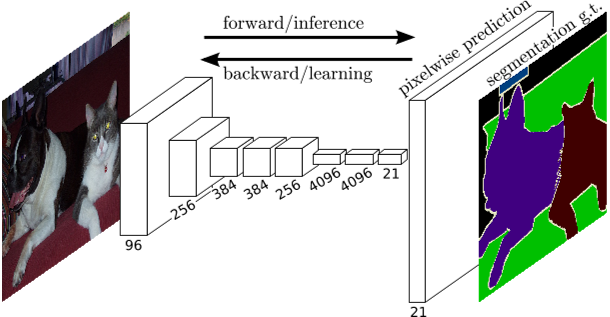
\includegraphics[width=0.49\linewidth]{images/fullCNN}
        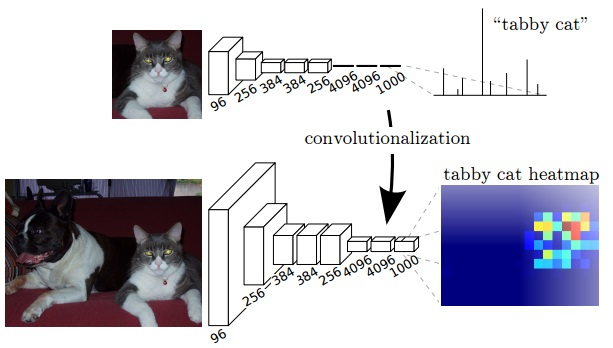
\includegraphics[width=0.49\linewidth]{images/FCN_heatmap}
        
        \caption{Fully CNN can learn to make prediction pixel-per-pixel for semantic segmentation}
        \label{fullCNN}
    \end{figure}
    
    The main difference between a fully CNN and a regular CNN, is that there is no fully connected layers in a fully CNN. So in every layer, we learn filters. 
    
     The number of kernels for every convolution layer equals the product of layers outputs to the number of input images.
    
    
end-to-end\\
receptive field : parameter, filter size. Region in which the neuron is connected\\
VGG net, GoogLeNet\\
Fully convolutional networks\\
skip architecure\\

mean IU(Intersection over union) segmentation : true positive / (true positive + false positive + false negative) \\


\subsection{Topology Aware Fully Convolutional Networks For Histology Gland Segmentation\cite{FCN_Gland_Segmentation}}
	
    We just saw how to train a CNN end-to-end in order to segment an image. The main disadvantage of using CNN with cross-entropy loss instead of using other methods is the fact that CNN does not have any prior knowledge about the dataset. He's just trying to solve an optimization problem in the same way that he'll solve it for any other dataset. 
    But introducing prior knowledge on a CNN, is not something impossible. One way to do it is to introduce prior knowledge in the loss function. 
    
    The paper \cite{FCN_Gland_Segmentation} propose different loss function which introduce prior knowledge in order to learn more efficiently the segmentation.
	
    They applied their methods for Histology Gland Segmentation. Given an input image, the goal is to identify the 3 different region : the background, the boundary around the gland, the inside glandular lumen.
    
     \begin{figure}
    	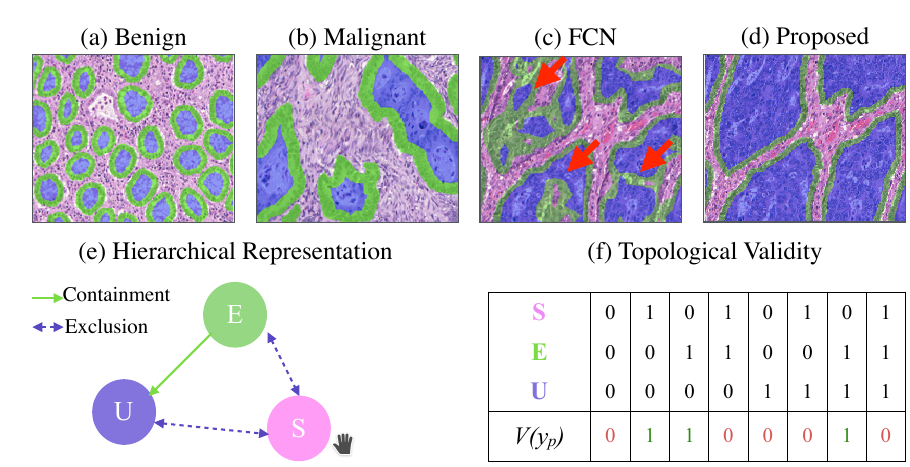
\includegraphics[width=\linewidth]{images/multiRegionGlandRepresentation}
        \label{MultiRegionGlandRepresentation}
        \caption{Multi region gland representation}
    \end{figure}
    
    Instead of using a Fully Convolutional Network per-pixel loss (cross entropy) : 
    
    \begin{center}
      \begin{align}
          \theta^* = \argmin_\theta \sum_{n=1}^N \Loss(x^{(n)};\theta) \\
          \Loss(x^{(n)};\theta) = \sum_{p\in\Omega}\sum_{r=1}^L -y_p^r log P(y_p^r = 1 | x_p; \theta)\\
          P(y_p^r = 1 | x_p; \theta) = \frac{exp(a_r(x_p}{\sum_{k=1}^L exp(a_k(x_p))}
      \end{align}
    \end{center}
    
    , they introduced hierarchical relations between region labels. Therefore, the loss function to optimize became : 
    \begin{align*}
    	\theta^* = \argmin_\theta \sum_{n=1}^N \alpha_1 \Loss_T(x^{(n)}; \theta) + \alpha_2 \Loss_S(x^{(n)}; \theta);
    \end{align*}
    
    Where $\Loss_T$ and $\Loss_S$ refer, in order, to the pixel-level loss functions that encode the topological relations betweens labels and the smoothness constraints. $\alpha_1$ and $\alpha_2$ are user-defined weights used to balance the contribution of each prior.
    
    $\Loss_T$ must be defined such that the network is trained, not only to penalize incorrect label assignment but also to penalize incorrect label hierarchy. For example, if we want a region U, to be contained in a region E, we want of course $P(y_p^U=1)$ to be high, but we also want $P(y_p^E=1)$ and $P(y_p^S=1)$ to be high (S is the background, cf figure \ref{MultiRegionGlandRepresentation}). That's why they defined the following unary loss : 
    \begin{align}
    	P(y_p | x_p; \theta) = 1/Z * \prod_{r=1}^L exp(a_r(x_p)) x y_p^r * V(y_p), Z =\sum_{r=1}^L P(y_p^r | x_p; \theta) 
    \end{align}
    
    
    
    
    